%\mbox{ \,} \\ \smallskip

Let
$\alpha_{act}=2\sqrt{2/5} \simeq 1.2649$.
%$\alpha_{act}{\simeq}1.2649$:

\begin{proposition}
The motion of the ACT Intouchpoints is as follows:

\begin{itemize}
    \item $a/b<\alpha_{act}$: monotonic in the direction of $P_1(t)$.
    \item $a/b=\alpha_{act}$: monotonic in the direction of $P_1(t)$, except for two instantaneous stops when passing at EB top and bottom vertices.
    \item $a/b>\alpha_{act}$:  non-monotonic with four reversals of velocity, a first (resp. second) pair of reversals near the EB's top (resp. bottom) vertex Figure~\ref{fig:act_intouch}.
\end{itemize}
\end{proposition}

\begin{proof}
 
As before, let a 3-periodic $P_1P_2P_3$ be parametrized by a leading vertex $$P_1(t)= (x_1, y_1) = (a\cos t, b\sin t).$$ 
%The ``enslaved'' vertices $P_2(t)$ and $P_3(t)$ are computed explicitly   in \cite{garcia2019-incenter}.  \textcolor{red}{The expressions
%for their coordinates involve double square roots on the coordinate $x_1$ so these points are constructible by ruler and compass\footnote{\textcolor{red}{The parameterization in $t$ is used to generate all the videos in the playlist.}}}.
%
Its ACT $P_i$' is given by double-length reflections of $P_i$ about the Barycenter $X_2$ \cite{mw}. Taking the ACT as the reference triangle, use Intouchpoint Trilinears $0:s_1s_3/(s_1-s_2+s_3)::$ \cite[Contact Triangle]{mw} to compute an Intouchpoint $i_1'(t)=(x_1(t),y_1(t))$ it follows that
$x_1'(t)\mid_{t=\frac{\pi}{2}}=0 $ is equivalent to $5 a^2-8b^2 =0$. This yields the result. 
\end{proof}

\noindent See \cite[PL\#09]{reznik2019-playlist-math-intelligencer} for an animation of the non-monotonic case. As we had been observing the EKG-like graph in Figure~\ref{fig:act-progress} (right), we stumbled upon an unexpected property, namely, the fixed linear relation between a 3-periodic vertex and its corresponding (opposite) Extouchpoint: 

\begin{proposition}
Let $P_i(t)=(x_i,y_i)$ be one of the 3-periodic vertices and $e_i=(x'_i,y'_i)$ be its corresponding Extouchpoint\footnote{Where $P_{i-1}(t)P_{i+1}(t)$ touch the Caustic.}  on the Caustic, where $a_c,b_c$ are the latter's semi-axes. Then\footnote{It can be shown \eqref{eqn:levi} also holds if $x',y'$ are the coordinates of an Excenter and $a_c,b_c$ are the semi-axes of the excentral locus, known to be an ellipse \cite{garcia2019-incenter}.}, for all $t$:
%
\begin{equation}
\frac{a}{b}\frac{y_i}{x_i}=\frac{a_c}{b_c}\frac{y'_i}{x'_i}
\label{eqn:levi}
\end{equation}
%
\noindent Equivalently, for $e_i(t')=[a_c \cos{t'},b_c\sin{t'}]$, then $\tan(t)=\tan(t')$, i.e., $t'=t{\pm}\pi$.
\label{lem:extouch}
\end{proposition}

\begin{proof}
This property follows directly\footnote{We thank A. Akopyan for pointing this out.} from \cite[Lemma 3]{levi2007-poncelet-grid}.
\end{proof}

In fact,  more general properties of the 
``Poncelet grid'' are described in 
the reference above. The  result reported here is a particular case and can also be demonstrated by simplifying rather long symbolic parametrics with a Computer Algebra System (CAS). 
 


Furthermore, since  $a_c=(\delta-{b}^{2})a/c^2$ and $b_c=({a}^{2}-\delta)b/c^2$ \cite{garcia2020-new-properties}: 
%
\begin{equation}
\frac{y}{x}=\left(\frac{\delta-b^2}{a^2-\delta}\right)\frac{y'}{x'}
\end{equation}
%
\begin{figure}
    \centering
    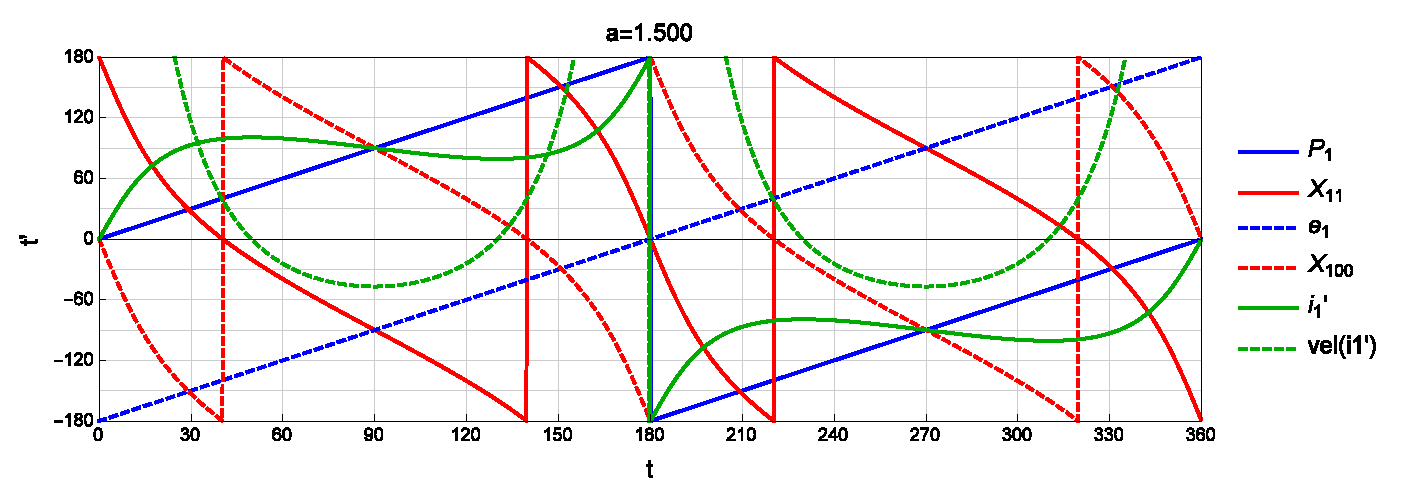
\includegraphics[width=\textwidth]{pics/1110_act_progress_clean_15.eps}
    \caption{The ``EKG'' of ACT motion, to be interpreted as a flat torus. On the horizontal axis is parameter $t$ of $P_1(t)=[a\cos(t),b\sin(t)]$, with $a/b=1.5$. On the vertical is the $t$ parameter for $P_1,X_{11},X_{100}$ and an ACT Intouchpoint $i_1'$. These all lie on the EB and are shown blue, red, dashed red, and green, respectively. Also shown is Extouchpoint $e_1$ on the Caustic (dashed blue). Just for it, the vertical axis represents $t'$ in $e_1=[a_c\cos(t'),b_c\sin(t')]$, where $a_c,b_c$ are the Caustic semi-axes. By Proposition~\ref{lem:extouch}, $t'=t{\pm}\pi$. Notice the only non-monotonic motion is that of $i_1'$ since $a/b>\alpha_{act}{\simeq}1.265$. To see this, a $\text{vel}(i_1')$ of its velocity is also shown (dashed green), containing two negative regions corresponding to 4 critical points of position. For $vel(i_1')$ ignore units and the fact that values near $0^\circ,180^\circ$ are not shown, these are all positive and above the vertical scale.}
    \label{fig:act-progress}
\end{figure}